\subsection{Polarizing Magnet and the Cryostat}

In {\tt CLAS12} the polarizing magnetic field will be provided by the 
superconducting solenoid of the central detector. The target will be 
placed in the center of a warm solenoid bore with the center of the target 
at approximately 2~m away from the upstream entrance of the magnet.  
A diagram for such a setup is shown in Fig.~\ref{target-in}.

The solenoid magnet is in the design stage, and not all parameters are well 
known at the moment. Some additional correction coils might be necessary to 
improve the field uniformity around the target cell. The DNP method requires 
that the target material is placed in a magnetic field of uniformity 
$\frac{\Delta B}{B}$ $<$ 10$^{-4}$. The current magnet design provides for 
such a region of field uniformity in a cylinder of 30~mm in diameter and 
100~mm in length. Some properties of the magnet are listed in 
Table~\ref{Magnet}. 

%%%%%%%%%%%%%%%%%%%%%%%%%%%%%%%%%%%%%%%%%%%%%%%%%%%%%%%%%%%%%%%%%%%%%%%
\begin{figure}[htbp]
\centering
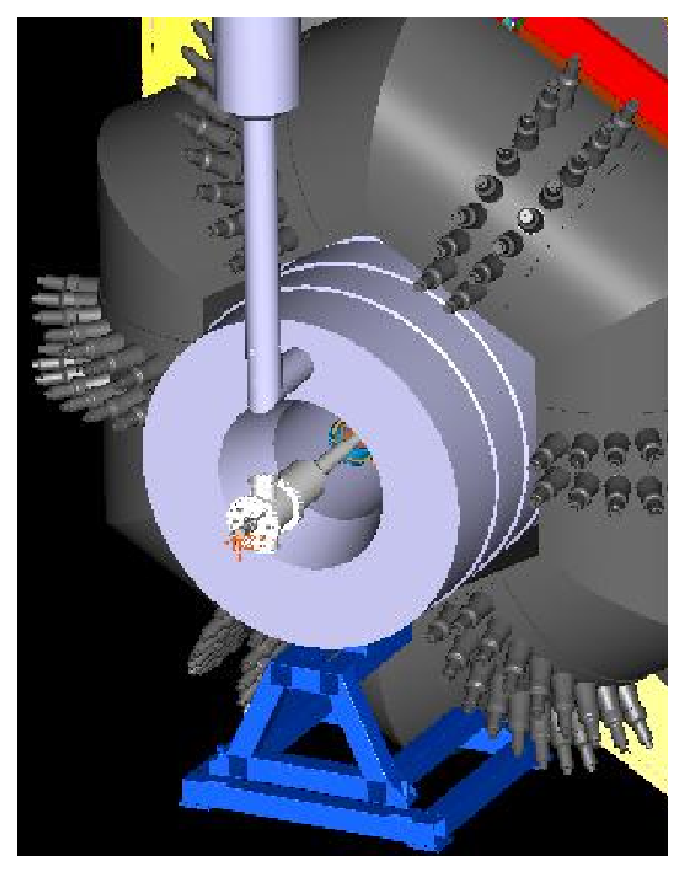
\includegraphics[width=0.6\textwidth]{\plots/target-in.eps}
\caption{\small{A schematic drawing of the polarized target cryostat inside 
of the solenoid magnet.}}
\label{target-in}
\end{figure}
%%%%%%%%%%%%%%%%%%%%%%%%%%%%%%%%%%%%%%%%%%%%%%%%%%%%%%%%%%%%%%%%%%%%%%%

%%%%%%%%%%%%%%%%%%%%%%%%%%%%%%%%%%%%%%%%%%%%%%%%%%%%%%%%%%%%%%%%%%%%%%%%%%%
\begin{table}[htbp]
\begin{center}
\begin{tabular}{|cc|} \hline
Type           & Superconducting solenoid \\ \hline 
Aperture       & 0.78~m warm bore \\ \hline
Central field  & 2.5-5~T \\ \hline
Dimensions     & 1.10~m OD x 0.78~m ID x 1.800~m long \\ \hline
Region of $\frac{\Delta B}{B} < 10^{-4}$ &  cylinder: 10~cm long, 3~cm OD \\ \hline
\end{tabular}
\end{center}
\caption{\small{Solenoid magnet properties.}}
\label{Magnet}
\end{table}
%%%%%%%%%%%%%%%%%%%%%%%%%%%%%%%%%%%%%%%%%%%%%%%%%%%%%%%%%%%%%%%%%%%%%%%%%%%

%%%%%%%%%%%%%%%%%%%%%%%%%%%%%%%%%%%%%%%%%%%%%%%%%%%%%%%%%%%%%%%%%%%%%%%%%%%
\begin{figure}[ht]
\includegraphics[width=12cm, angle=90]{\plots/ConceptCutaway1.eps}
\caption{A schematic drawing of the polarized solid target cryostat and 
target insert for {\tt CLAS12}.} 
\label{cryostat}
\end{figure}
%%%%%%%%%%%%%%%%%%%%%%%%%%%%%%%%%%%%%%%%%%%%%%%%%%%%%%%%%%%%%%%%%%%%%%%%%%%

The target cryostat will house the evaporation refrigerator, the target 
insert and some instrumentation necessary for the microwave and NMR 
operations. The cryostat needs to be designed to allow its operation in a 
warm bore magnetic field. The 'target ladder' used in the previous experiments 
is not possible with this geometry. The cryostat will contain a single cell 
filled with a polarizable target material. It would also be possible to 
place a carbon target upstream or downstream of the polarized target cell.
A conceptual design of the target cryostat is shown in Fig.~\ref{cryostat}.
The main component of the cryostat is a $^{4}$He evaporation refrigerator. 
The refrigerator is inserted horizontally through a pumping tube between the 
pumps and the evaporation chamber. One important difference between this 
design and the previously used polarized target in Hall B is that the 
refrigerator will be residing along the beam line, so that the amount of 
materials in the way of the beam needs to be  minimized. 
 
The evaporation chamber will be situated in the bore of the magnet.  The 
silicon vertex tracker (SVT) will also be installed in the magnet bore, 
surrounding the target, and imposing constraints on the chamber dimensions. 
The constraining radius of the SVT is 40.25~mm in the current design, which 
is NOT compatible with the current target design, in which the minimum outer 
diameter of the target cryostat is 10~cm.  This volume of the cryostat will 
contain the outer vacuum space, heat shield and the evaporation chamber. 
Diagrams of the cryostat section surrounded by the SVT planes are shown in 
Fig.~\ref{target-svt}. To make this picture possible, the cryostat diameter 
had to be shrunk to 7.6~cm.

%%%%%%%%%%%%%%%%%%%%%%%%%%%%%%%%%%%%%%%%%%%%%%%%%%%%%%%%%%%%%%%%%%%%%%%%%%%
\begin{figure}[h]
\begin{center}
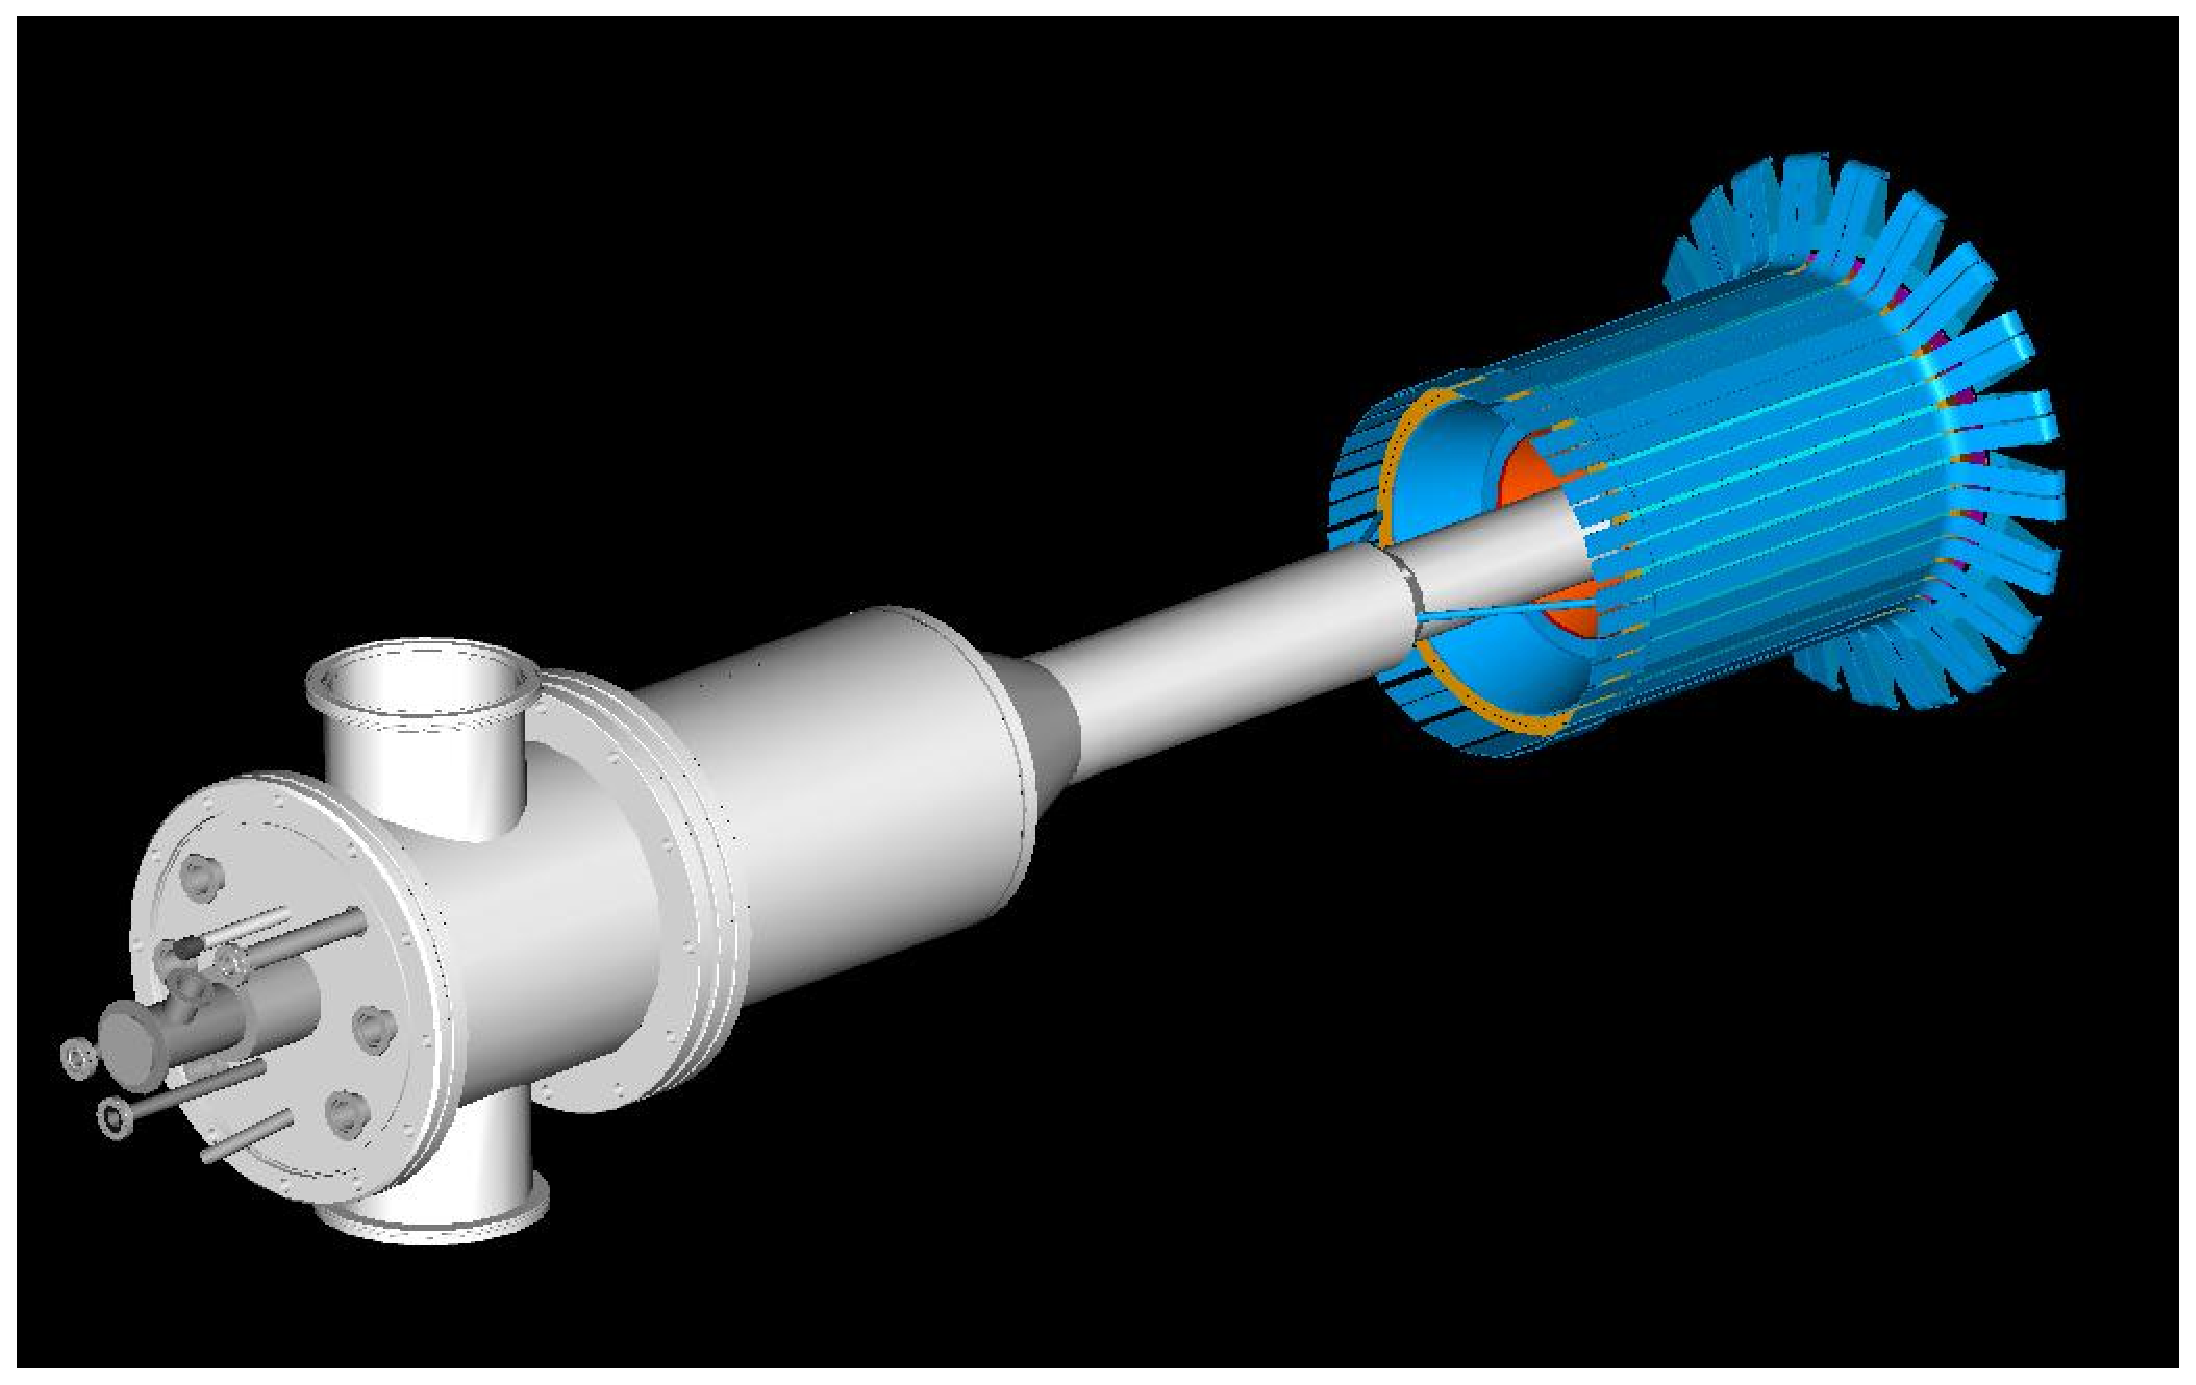
\includegraphics[width=4in]{\plots/target-svt2.eps}
\includegraphics[width=4in]{\plots/target-svt.eps}
\caption{Diagrams of the target cryostat surrounded by 
the SVT planes.}
\end{center}
\label{target-svt} 
\end{figure}
%%%%%%%%%%%%%%%%%%%%%%%%%%%%%%%%%%%%%%%%%%%%%%%%%%%%%%%%%%%%%%%%%%%%%%%%%%%

%%%%%%%%%%%%%%%%%%%%%%%%%%%%%%%%%%%%%%%%%%%%%%%%%%%%%%%%%%%%%%%%%%%%%%%%%%%
\begin{table}[hbt]
\begin{center}
\begin{tabular}{|ccc|} \hline
Name   & Material  & Dimensions  \\
\hline 
Outer Vacuum Jacket & Al & 0.5 mm \\
\hline
Heat Shield & Al & 0.5 mm \\
\hline
Cup Wall & Kel-F & 0.5 mm\\
\hline
Cup/Cell Windows & Al& 0.025 mm \\
\hline
Cell & Kel-F/torlon & 0.3 mm\\
\hline
\end{tabular}
\end{center}
\caption{New cryostat and insert design parameters}
\label{fridge}
\end{table} 
%%%%%%%%%%%%%%%%%%%%%%%%%%%%%%%%%%%%%%%%%%%%%%%%%%%%%%%%%%%%%%%%%%%%%%%%%%%
 
\clearpage

\subsection{Target Insert, Cells, $\mu$-waves, and NMR}

 The target material will be placed in the cell inside of a cup, with both 
containers made of hydrogen free plastic. The cup will be attached to a thin 
aluminum structure that can be inserted through the beam tube. The schematic 
of the insert is shown on the bottom of Fig.~\ref{cryostat}.  The dimensions 
of the target cell are determined by the size of the region of field 
uniformity, and geometric constraints of the cryostat. The cup will have an 
opening on the top for the LHe fill, while the cell will have small holes so 
that the target material will be sitting in a bath of LHe, while also being 
showered by LHe coming from the run valve. The flow of LHe in the cryostat 
will be maintained by a series of pumps located outside of the cryostat. The 
entrance and exit windows of the target cell and cup could be made out of 
thin aluminum or Kapton foils. The microwave radiation needed to polarize 
the target will be guided through a designated waveguide inserted through the 
upstream entrance window of the cryostat.  The guide will have a slit directly 
underneath the target cup, providing continuous microwave radiation directed 
at the  target cell. With this arrangement, the target cup will act as a 
resonating cavity.     

Ammonia and deuterated ammonia will be used as target material with the 
electron beam and {\tt CLAS12}. (We will also investigate the possibility of 
using $^6$LiH(D) as a target material). Ammonia will be frozen and broken up 
into small beads (to optimize the cooling surface) which fill the target cup.
Some parameters of frozen ammonia are listed in Table~\ref{ammo}.  These 
targets offer high polarization, good resistance to radiation damage, and a 
relatively high ratio of polarizable nucleons per total number of nucleons. 
With the goal luminosity, $L$, of 1$\times$10$^{35}$~cm$^{-2}$s$^{-1}$ and the 
tentative target dimensions of 3.0~cm in diameter and 3.3~cm in length, we can 
estimate the rate of charge accumulation, $J$.  We estimate the packing factor 
to be  $f_{\mathrm eff} \sim$ 0.6.

\begin{eqnarray}
J &=& f_{\mathrm eff}\times l \times \rho \times N_A \times N_{nucl} \times (1 mole/17g) \times L\\ \nonumber
J &=&0.6 \times 3.3 \times 0.91 \times  (1 mole/17g) \times 6.02\times 10^{23} \times 17 \times 10^{35}\\ \nonumber
J &=& 9.22 \times 10^{10} e^-/s\\ \nonumber
I &=& J\times 1.60 \times 10^{-19} C/e-) = 14.7 \times 10^{-9} A
\end{eqnarray}
Compared to the existing target (4~nA current, 1-cm long) this represents an 
increase by a factor of $\sim$12. 

%%%%%%%%%%%%%%%%%%%%%%%%%%%%%%%%%%%%%%%%%%%%%%%%%%%%%%%%%%%%%%%%%%%%%%%%%%%
\begin{table}[hbt]
%\centerline{\begin{tabular}{cc}\hline
\begin{center}
\begin{tabular}{|cc|} 
\hline
Chemical Structure  & NH$_3$(ND$_3$)   \\
\hline
Target Diameter     & 3 cm \\
\hline
Target Length       & 3.3 cm \\
\hline
Density             & 0.917(1.056) g/cm$^3$  \\
\hline
Dilution Factor     & $\approx 0.15 (0.22)$ \\
\hline
Packing Factor      & $\approx$ 0.6\\
\hline
\end{tabular}
\end{center}
\caption{Some parameters of the ammonia targets}
\label{ammo}
\end{table}
%%%%%%%%%%%%%%%%%%%%%%%%%%%%%%%%%%%%%%%%%%%%%%%%%%%%%%%%%%%%%%%%%%%%%%%%%%%

The target polarization will be monitored during the run via the NMR system, 
in the field of solenoid magnet. The calibration of the proton NMR can be 
done by measurements of polarization in thermal equilibrium, taken with the 
polarizing magnet. In cases when the deuteron signal is too small for the 
thermal equilibrium measurement, the polarization can be monitored through 
the ratio of the two peaks of the NMR signal ($R$-ratio method).  The target 
cell size in the current design is relatively large, which will allow for 
placement of the coils inside of the cell resulting in a measurable thermal 
equilibrium signal, so the polarization of deuterium will be monitored by 
the area and ratio methods.

\subsection{Heat Load and Pumping requirements}

Assuming the energy loss of 2~MeV/g/cm$^2$, the heat load due to the beam 
will be:

\begin{equation}
J \times (2\times10^6 eV/g/cm^2)\times \rho \times f_{\mathrm eff}\times l 
\times (1.602\times 10^{-19}J/eV) = 0.053 W
\end{equation}

The heat load due to the microwaves is more difficult to estimate. Systems 
with movable target ladders, such as the existing Hall B polarized target 
and the UVa-SLAC target, use horns to direct microwaves toward the target. 
In these systems the target is not located inside a microwave cavity and 
the microwave power delivered to the target region is typically 0.5~W to 1~W. 
In systems with a single, fixed target it is possible to locate the target 
inside a multi-mode cavity with highly conductive walls.  The Yale-SLAC 
polarized target operated with 0.5~W of microwave power even though the 
volume of target material was relatively large (25~cm$^3$).  A value of 0.5~W 
of microwave power should be a relatively safe assumption for this target.
The total heat load is expected to be 0.55~W.

The heat of evaporation of $^4$He at 1 K is approximately 80~J/mole.  To 
provide 0.55~W, a flow rate of 0.0069~moles/s will be required.  At 1.0~K 
the vapor pressure of $^4$He is 0.160~mb.  The displacement of the pumping 
system will be:

\begin{equation}
.0069 mole/s \times (22.4 l/mole)\times (1 b/0.160 \times 10^{-3} b) 
= 966 l/s = 3480 m^3/hr.
\end{equation}

The measured pumping speed for the existing Hall B polarized target pump set 
is 3300~m$^3$/hr.  A larger pumping system will be required.  It is desirable 
to use hermetically sealed pumps in order to avoid contamination of helium 
gas that is returned to the liquefier. A system based on the WKP6000 AM 
series (Pfeiffer) would be suitable.

